\documentclass[addpoints,12pt]{exam}
\usepackage{amsmath, amssymb}
\linespread{1.1}
\usepackage{graphicx}
\usepackage[T1]{fontenc}
\boxedpoints
\pointsinmargin

\printanswers

\pagestyle{headandfoot}
\runningheadrule
\runningheader{Econ 103}
              {Midterm I, Page \thepage\ of \numpages}
              {February 16th, 2016}

\runningfooter{Name: \rule{5cm}{0.4pt}}{}{Student ID \#: \rule{5cm}{0.4pt}}


%%%%%%%%%%%%%%%%%%%%%%%%%%%%%%%%%%%%%%%%%%%%%%%%%%%%%%%%%%%%%%%
\begin{document}

\begin{center}
\textsc{\large First Midterm Examination\\ \normalsize Econ 103, Statistics for Economists \\ \vspace{0.5em} February 16th, 2016}

\vspace{2em}

\fbox{\begin{minipage}{0.5\textwidth}
\normalsize\textbf{You will have 70 minutes to complete this exam.
Graphing calculators, notes, and textbooks are not permitted. }\end{minipage}}


\end{center}
%%%%%%%%%%%%%%%%%%%%%%%%%%%%%%%%%%%%%%%%%%%%%%%%%%%%%%%%%%%%%%%


\vspace{2em}
\begin{center}
  \fbox{\fbox{\parbox{5.5in}{\centering
        I pledge that, in taking and preparing for this exam, I have abided by the University of Pennsylvania's Code of Academic Integrity. I am aware that any violations of the code will result in a failing grade for this course.}}}
\end{center}
\vspace{0.2in}
\makebox[\textwidth]{Name:\enspace\hrulefill}

\vspace{0.2in}

\noindent\makebox[\textwidth]{Signature:\enspace\hrulefill}

\vspace{0.2in}

\noindent\makebox[0.47\textwidth]{Student ID \#:\enspace\hrulefill}
\hfill
\makebox[0.47\textwidth]{Recitation \#:\enspace\hrulefill}

\vspace{2em}

\begin{center}
  \gradetable[h][questions]
\end{center}

\vspace{2em}

\paragraph{Instructions:} Answer all questions in the space provided, continuing on the back of the page if you run out of space. Show your work for full credit but be aware that writing down irrelevant information will not gain you points. Be sure to sign the academic integrity statement above and to write your name and student ID number on \emph{each page} in the space provided. Make sure that you have all pages of the exam before starting.

\paragraph{Warning:} If you continue writing after we call time, even if this is only to fill in your name, twenty-five points will be deducted from your final score. In addition, two points will be deducted for each page on which you do not write your name and student ID. 

%%%%%%%%%%%%%%%%%%%%%%%%%%%%%%%%%%%%%%%%%%%%%%%%%%%%%%%%%%%%%%%
\newpage
\begin{questions}

  \question The dataframe \texttt{Austin} describes 4499 students who entered the UT Austin in 2000:
  \small
\begin{verbatim}
  SATv SATq          School    GPA
1  690  580        BUSINESS 3.8235
2  530  710 NATURAL SCIENCE 3.5338
3  610  700 NATURAL SCIENCE 3.3679
4  730  700     ENGINEERING 3.3437
5  700  710 NATURAL SCIENCE 3.7205
6  540  690    LIBERAL ARTS 2.6851
\end{verbatim}
\normalsize
Columns 1--2 are SAT \emph{verbal} and \emph{quantitative} scores (out of 800), \texttt{School} indicates if a student is in the school of \texttt{BUSINESS}, \texttt{ENGINEERING}, \texttt{LIBERAL ARTS} or \texttt{NATURAL SCIENCE}, and \texttt{GPA} gives GPA at graduation (out of 4.0).
\begin{parts}
%\part[2] Give the full R command that I used to display the first six rows of \texttt{Austin} above.
%  \begin{solution}
%    \texttt{head(Austin)}
%  \end{solution}
\part[2] The first thing I did was compute some basic descriptive statistics:
\small
\begin{verbatim}
      SATv            SATq                   School          GPA       
 Min.   :270.0   Min.   :320.0   BUSINESS       : 832   Min.   :1.837  
 1st Qu.:540.0   1st Qu.:570.0   ENGINEERING    : 695   1st Qu.:2.846  
 Median :590.0   Median :630.0   LIBERAL ARTS   :1847   Median :3.238  
 Mean   :595.6   Mean   :624.9   NATURAL SCIENCE:1125   Mean   :3.195  
 3rd Qu.:650.0   3rd Qu.:680.0                          3rd Qu.:3.582  
 Max.   :800.0   Max.   :800.0                          Max.   :4.000  
\end{verbatim}
\normalsize
I created these results with a single line of R code. What was it?
\begin{solution}[0.75in]
  \texttt{summary(Austin)}
\end{solution}
%\part[3] Suppose I wanted to determine which shows more spread: SAT verbal scores or GPA.
%Would a comparison of interquartile ranges suffice?
%Why or why not?
%\begin{solution}
%  No: the units would not be comparable since GPA is out of 4 while SAT is out of 800.
%\end{solution}
%  \part[3] I wanted to know the proportion of students in the dataset in each school, so I constructed a one-way cross-tab in \emph{percents}:
%  \small
%  \begin{verbatim}
%BUSINESS     ENGINEERING    LIBERAL ARTS NATURAL SCIENCE 
%    0.18            0.15            0.41            0.25  
%  \end{verbatim}
%  \normalsize 
%  \vspace{-1.5em}
%  Provide a single line of R code to generate these results using \texttt{Austin}. 
%  \begin{solution}
%    \texttt{prop.table(table(Austin\$School))}
%  \end{solution}
  \part[3] I decided to calculate each student's \emph{combined} SAT score and add it as an additional column in \texttt{Austin}.
  After doing this, the first few rows of \texttt{Austin} were:
  \small
\begin{verbatim}
  SATv SATq          School    GPA SATc
1  690  580        BUSINESS 3.8235 1270
2  530  710 NATURAL SCIENCE 3.5338 1240
3  610  700 NATURAL SCIENCE 3.3679 1310
4  730  700     ENGINEERING 3.3437 1430
5  700  710 NATURAL SCIENCE 3.7205 1410
6  540  690    LIBERAL ARTS 2.6851 1230
\end{verbatim}
\normalsize
Write a single line of R code to compute \texttt{SATc} and add it to \texttt{Austin}.
\begin{solution}[0.75in]
  If \texttt{Austin} is a \texttt{data.table}, we add the column with:
  \texttt{Austin[ , SATc := SATv + SATq]}
  If \texttt{Austin} is a \texttt{data.frame}, we do:
  \texttt{Austin\$SATc <- Austin\$SATv + Austin\$SATq}
\end{solution}
\part[3] The next thing I did was to create histograms of GPA and combined SAT scores:
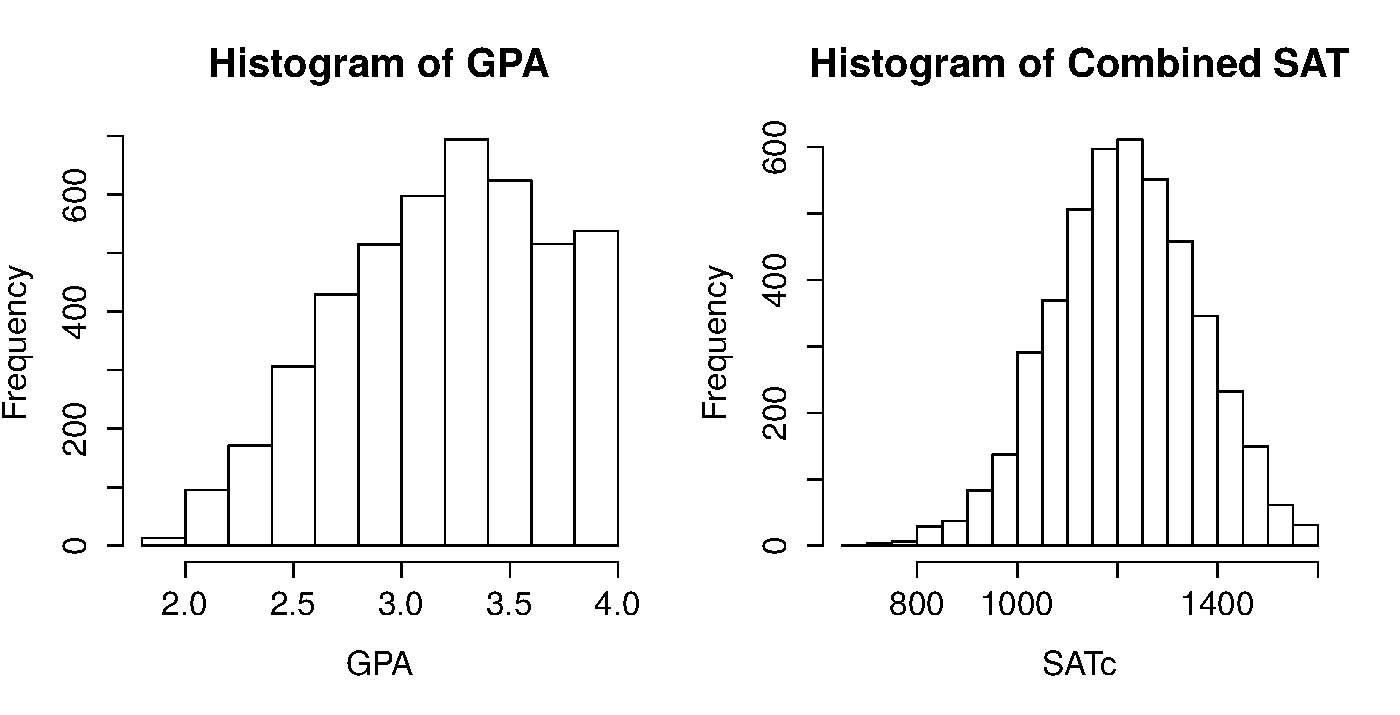
\includegraphics[scale = 0.5]{GPA_SAT_hist.pdf}

Give the full R command I used to make the histogram for \emph{GPA}.
Don't forget to include the title and label for the $x$-axis.
\begin{solution}[0.75in]
  \texttt{hist(Austin\$GPA, xlab = `GPA', main = `Histogram of GPA')}
\end{solution}

\part[3] Is there any evidence of skewness in \texttt{GPA} or \texttt{SATc}? Explain briefly.
\begin{solution}[0.75in]
  \texttt{SATc} is symmetric while \texttt{GPA} is \emph{left}-skewed since the grade point averages ``pile up'' at 4.0 at the upper end.
\end{solution}
\part[3] I was interested to see whether GPA varies by school so I produced this plot:
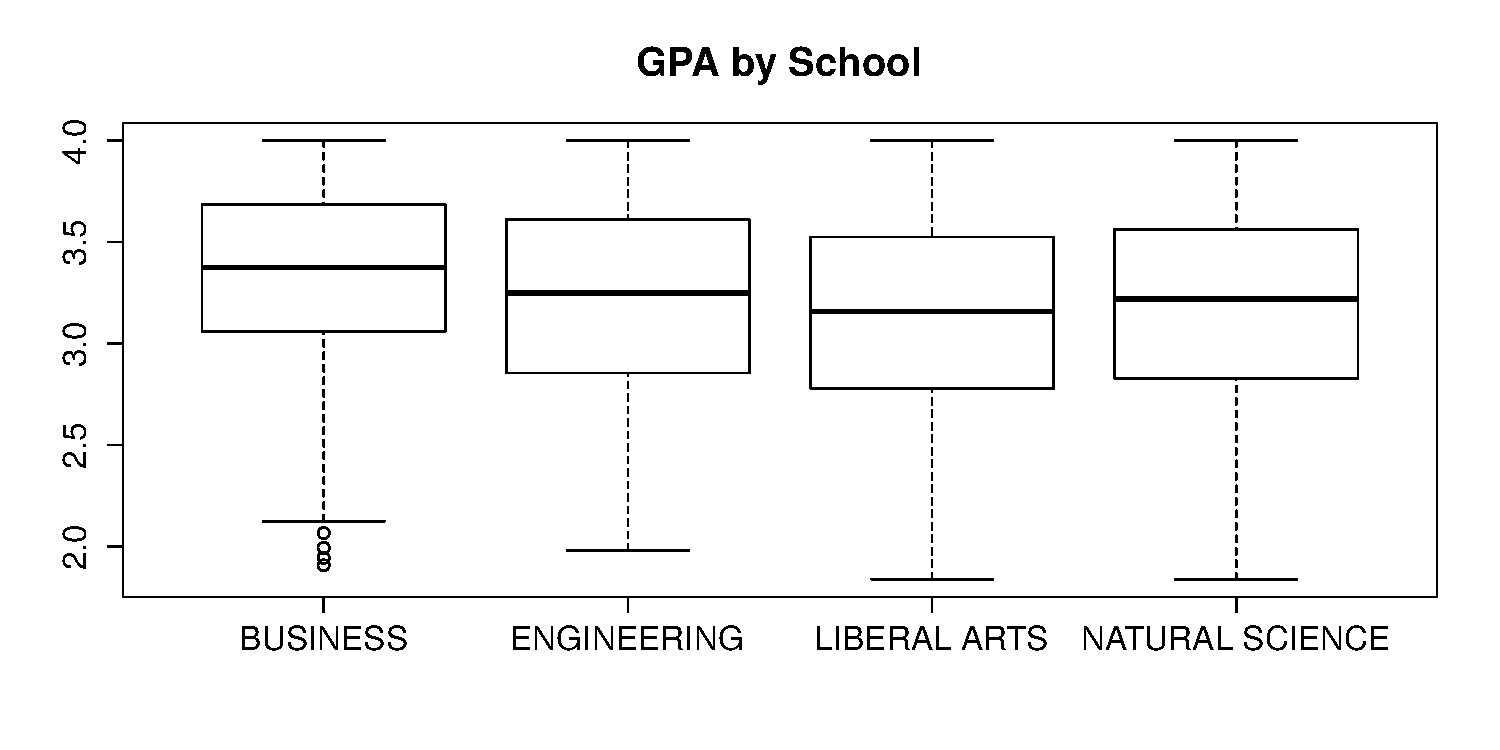
\includegraphics[scale = 0.5]{GPA_boxplot.pdf}

Write out the full R command that I used. Don't forget the plot title. 
\begin{solution}[0.75in]
  \texttt{boxplot(GPA\textasciitilde School, data = Austin, main = `GPA by School')}
\end{solution}

\part[3] What are the ``little circles'' that appear in the preceding plot?
Explain briefly.
\begin{solution}[1in]
  These represent outliers: students with extremely low GPAs relative to the other students in the Business school.
\end{solution}
\part[3] Next I calculate the average \emph{combined} SAT score for students of each school:
\small
\begin{verbatim}
  Austin$School: BUSINESS
  [1] 1230.288
  ------------------------------------------------------------------- 
  Austin$School: ENGINEERING
  [1] 1281.554
  ------------------------------------------------------------------- 
  Austin$School: LIBERAL ARTS
  [1] 1187.163
  ------------------------------------------------------------------- 
  Austin$School: NATURAL SCIENCE
  [1] 1230.338
\end{verbatim}
\normalsize
What command did I use?
\begin{solution}[0.75in]
  The syntax to get the equivalent output is:
  \texttt{Austin[ , mean(SATc), by = School]}
  The output found on this exam was produced by the \texttt{by} command (which is no longer covered):
  \texttt{by(Austin\$SATc, Austin\$School, mean)}
\end{solution}
\uplevel{\emph{\textbf{Use these statistics to answer the remaining parts:}}
\begin{center}
\begin{tabular}[h]{|r|cc|}
  \hline
  &\texttt{GPA} & \texttt{SATc}\\
  \hline
  Mean & 3.2 & 1220\\
  S.D. & 0.5 & 145\\
  Cov. & \multicolumn{2}{c|}{29}\\
  \hline
\end{tabular}\end{center}}
\part[3] Based on the sample z-scores, which is more ``extreme'' in this dataset: a GPA of 3.7 or a combined SAT score of 1400?
Explain briefly.
\begin{solution}[1in]
  A GPA of 3.7 is one standard deviation above the mean GPA while an SAT score of 1400 is more than one standard deviation about the mean SAT score, so the latter is ``more extreme.''
\end{solution}
\part[3] Calculate the sample correlation between \texttt{GPA} and \texttt{SATc}.
\begin{solution}[1in]
  $r_{XY} = s_{XY}/(s_X s_Y) = 29/(0.5 \times 145) = 0.4$
\end{solution}
\part[3] Calculate the slope of the regression line when \texttt{SATc} is used to predict \texttt{GPA}
\begin{solution}[1in]
  $b = s_{XY} / s_X^2 = 29/(145^2) \approx 0.0014$ 
\end{solution}
\part[3] Continuing from the previous part, calculate the \emph{intercept} of the regression line.
\begin{solution}[1in]
  $a = \bar{y} - b \bar{x} = 3.2 - 0.0014 \times 1220 \approx 1.5$
\end{solution}
\part[3] Hazel's combined SAT score was 1450.
Based on the regression from the preceding two parts, what GPA would we predict for her?
\begin{solution}[1in]
  $\widehat{y} = 1.5 + 0.0014 \times 1450 = 3.53$
\end{solution}
\end{parts}


\question[15] Write an R function called \texttt{skew} that calculates the skewness of a sample of observations.
Your function should take a single argument, the vector of data \texttt{x}, and return the skewness of this vector.
Your function should account for the possibility that \texttt{x} may have missing values and drop them before carrying out the calculation.
\begin{solution}[3.75in]
  There are various ways to do this. Here is perhaps the simplest:
  \begin{verbatim}
skew <- function(x){
  x <- x[!is.na(x)] 
  out <- mean((x - mean(x))^3) / (sd(x))^3
  return(out)
}
  \end{verbatim}
\end{solution}

\question This problem asks you to construct arbitrage strategies.
While the example from class involved buying only, in general an arbitrage strategy can involve buying \emph{and or} selling. This question concerns the ongoing election to become the presidential candidate for the Democratic Party (who will `win the nomination'). To decide who wins the nomination, there are a series of votes in each state. Parts (a) and (b) concern who wins the overall nomination, and parts (c) and (d) concern who will win the next two state votes, in Nevada and South Carolina.

\begin{parts}
  \part[5] Rodrigo wonders which of the two remaining Democratic candidates, Sanders or Clinton, will win the nomination so he checks his two prediction markets.
On one he finds contract C trading at \$0.63 that pays \$1 if Clinton wins; on the other he finds contract S trading at \$0.48 that pays \$1 if Sanders wins.
Explain the probability rule these prices violate.
\begin{solution}[1in]
 The complement rule: since Sanders ($S$) and Clinton ($C$) are the only two candidates, we should have $P(C) + P(S) = 1$ but the prices of these contracts add up to \$1.11 which implies that the sum of the probabilities is 1.11!
\end{solution}

\part[5] Continuing from the previous part, construct an arbitrage strategy that Rodrigo could use to exploit the market mis-pricing.
Explain exactly what he should buy and/or sell and how much he will earn for each possible outcome.
\begin{solution}[1.5in]
  Rodrigo should \emph{sell} as many \emph{pairs} of B and S as he can afford.
  Consider a single pair.
  When he sells the pair he earns \$0.68 + \$0.48 = \$1.11. 
  Now, if Sanders wins Clinton doesn't so Rodrigo has to pay out \$1. 
  On the other hand if Clinton wins, then Sanders doesn't so Rodrigo has to pay out \$1. 
  Either way his net profit is \$0.11 per pair.
\end{solution}

\part[5] Later Rodrigo again checks both prediction markets.
On one he finds contract B trading at \$0.62 that pays \$1 if Clinton wins \emph{both} the Nevada and South Carolina primaries.
On the other he finds contract NV trading at \$0.55 that pays \$1 if Clinton wins the \emph{Nevada} primary. 
Explain the probability rule these prices violate.
\begin{solution}[1in]
  They violate the logical consequence rule.
  If Clinton wins \emph{both} of the next two primaries she \emph{must} have won the Nevada primary.
  Therefore the probability that she wins both primaries \emph{should not exceed} the probability that she wins the Nevada primary.
  The market price of B should not be greater than that of NV. 
\end{solution}

\newpage
\part[10] Continuing from the previous part, construct an arbitrage strategy that Rodrigo could use to exploit the market mis-pricing of contracts B and NV.
Explain exactly what he should buy and/or sell and how much he will earn for each possible outcome. Write no more than 5 bullet points. 
\begin{solution}[1.5in]
  Rodrigo should \emph{sell} B and \emph{buy} NV in equal numbers.
  Consider a single pair of contracts: one B sold and one NV bought.

  If Clinton wins both primaries, then in particular she wins Nevada. 
  In this case Rodrigo wins \$1 from NV which he bought for \$0.55 for a net gain of \$0.45. 
  But at the same time he has to pay out \$1 for B which he sold for \$0.62 for a net loss of \$0.38.
  All told his net gain is \$0.07.

  On the other hand, if Clinton does \emph{not} win both primaries then Rodrigo does not have to pay out on the B he sold: on this particular contract he nets the full sale price of \$0.62.
  Now there are two possibilities to consider regarding NV.
  If Clinton wins Nevada then Rodrigo wins \$1 from the NV contract that he bought for \$0.55, resulting in a net gain of \$0.45 from NH.
  In this case his total profit would be \$0.45 + \$0.62 = \$1.07 per pair.
  If Clinton does not win both primaries and \emph{loses} Nevada, then Rodrigo has a loss of \$0.55 from the NV he bought but still comes out ahead because he gains \$0.62 from the B he sold: his total profit is \$0.07 per pair.

  Thus, no matter what happens, Rodrigo is guaranteed to make a profit.
\end{solution}

\end{parts}

\newpage
\uplevel{\emph{This was an assigned homework problem from the text. I have re-phrased it slightly to make it easier to understand but the substance and solution are unchanged.}}

\question A plane has crashed in one of three possible locations: the mountains ($M$), the desert ($D$), or the sea ($S$).
Based on its flight path, experts have calculated the following prior probabilities that the plane is in each location: $P(M) = 0.5$, $P(D) = 0.3$ and $P(S) = 0.2$.
If we search the mountains then, given that the plane is actually there, we have a 30\% chance of \emph{failing} to find it.
If we search the desert then, given that the plane is actually there, we have a 20\% chance of \emph{failing} to find it.
Finally, if we search the sea then, given that the plane is actually there, we have a 90\% chance of \emph{failing} to find it. 
Naturally if the plane is \emph{not} in a particular location but we search for it there, we will not find it.
You may assume that searches in each location are independent.
Let $F_M$ be the event that we \emph{fail} to find the plane in the mountains.
Define $F_D$ and $F_S$ analogously.
\begin{parts}
  \part[10] We started by searching the mountains.
  We did not find the plane.
  What is the conditional probability that the plane is nevertheless in the mountains?
  Explain.
  \begin{solution}[2in]
    By Bayes' Rule: $P(M|F_M) = P(F_M|M)P(M)/P(F_M)$.
    We first calculate the denominator using the Law of Total Probability:
    \begin{eqnarray*}
      P(F_M) &=&  P(F_M|M)P(M) + P(F_M|M^C)P(M^C) \\
      &=& 0.3 \times 0.5 + 1 \times 0.5 = 0.15 + 0.5 = 0.65
    \end{eqnarray*}
    Hence, the desired probability is $15/65 = 3/13 \approx 0.23$.
  \end{solution}
\part[20] After failing to find the plane in the mountains, we searched the desert, and the sea.
  We did not find the plane in either location.
  After this more exhaustive search what is the conditional probability that the plane is in the mountains?
  Explain.
  \begin{solution}[2.75in]
    We are asked to calculate $P(M|F_M \cap F_D \cap F_S)$.
    By Bayes' rule, 
    $$P(M|F_M \cap F_D \cap F_S) = \frac{P(F_M \cap F_D \cap F_S|M)P(M)}{P(F_M \cap F_D \cap F_S)}$$
    Define the shorthand $A = F_M \cap F_D \cap F_S$. 
    By the Law of Total Probability
    \begin{eqnarray*}
      P(A) &=& P(A|M)P(M) + P(A|D)P(D) + P(A|S)P(S) \\
      &=& (0.3 \times 1 \times 1) \times 0.5 + (1 \times 0.2 \times 1) \times 0.3 + (1 \times 1 \times 0.9 ) \times 0.2 \\
      &=&  0.15 + 0.06 + 0.18 = 0.39
    \end{eqnarray*}
    using independence.
    Hence, the desired probability is $15/39 \approx 0.38$.
  \end{solution}
\end{parts}


\question Let $X$ be a random variable that equals the total number of heads that you get over four tosses of a fair coin and define $Y = 10X + 25$. 
\begin{parts}
  \part[5] Write out the support set and probability mass function of $X$.
  \begin{solution}[1.75in]
    The support set is $\left\{ 0,1,2,3,4 \right\}$.
    For the pmf, a correct answer either gives $p(x) = {4\choose x} (1/2)^x (1 - 1/2)^{4-x} = {4 \choose x}1/2^4$ or specifies the probabilities individually: $p(0) = 1/16$, $p(1) = 1/4$, $p(2) = 3/8$, $p(3) = 1/4$, $p(4) = 1/16$. 
  \end{solution}
  \part[5] Write out the cumulative distribution function of $X$. 
  \begin{solution}[1.75in]
    \[
      F(x_0) = \left\{
      \begin{array}{ll}
        0, & x_0 < 0 \\
        1/16, & 0 \leq x_0 < 1 \\
        5/16, & 1 \leq x_0 < 2 \\
        11/16, & 2 \leq x_0 < 3 \\
        15/16, & 3 \leq x_0 < 4 \\
        1, & x_0 \geq 4 
      \end{array}
      \right.
    \]
  \end{solution}
  \part[5] Calculate $E[X]$.
  \begin{solution}[1.75in]
    \begin{eqnarray*}
      E[X] &=& 0 \times p(0) + 1 \times p(1) + 2 \times p(2) + 3 \times p(3) + 4 \times p(4) \\
      &=& 1/4 + 2 \times 3/8 + 3 \times 1/4 + 4 \times 1/16  = 2
    \end{eqnarray*}
  \end{solution}
  \part[5] Calculate $E[X^2]$.
  \begin{solution}[1.75in]
    \begin{eqnarray*}
      E[X^2] &=& 0^2 \times p(0) + 1^2 \times p(1) + 2^2 \times p(2) + 3^2 \times p(3) + 4^2 \times p(4)\\
      &=& 1/4 + 4 \times 3/8 + 9 \times 1/4 + 16 \times 1/16  = 5
    \end{eqnarray*}
  \end{solution}
  \newpage
  \part[5] Calculate $Var(X)$.
  \begin{solution}[1.74in]
    By the shortcut formula $Var(X) = E[X^2] - E[X]^2 = 5 - 2^2 = 1$
  \end{solution}
  \part[5] Calculate $E[Y]$.
  \begin{solution}[1.75in]
    Since $E[aX + b] = a E[X] + b$, $E[Y] = 10 \times E[X] + 25 = 45$. 
  \end{solution}
  \part[5] Calculate $Var(Y)$.
  \begin{solution}[1.75in]
    Since $Var(aX + b) = a^2 Var(X)$, $Var(Y) = 100 \times Var(X) = 100$.
  \end{solution}
\end{parts}


\end{questions}

\end{document}
